

\documentclass[twocolumn,12pt,journal]{IEEEtran}
\usepackage{cite}
\usepackage{graphicx}

%\usepackage[backend=biber,style=ieee]{biblatex}
%\addbibresource{bibliography.bib}

\begin{document}

\title{CS3243: Introduction to AI\\ Let’s Play Tetris! }

\author{
  Group 13 \\
  Bjoern Jesper Andersson, Daniel Gunnarsson, \\Le Viet Bach, Low Yee Heng, Zeng Qingtao\\ 
  2014-0?-?? 
}

\maketitle

\begin{abstract}
    Skip?
\end{abstract}

\section{Introduction} 
Short description of what has been "solved".

\section{Strategy} 
    Use of duplicated state to evaluate moves
    Calculations used in the utility function
        Holes, wells, roughness etc.
    Parallel evaluations (Forks)
    Genetic algorithm to determine best weights
        Population, mutation rate etc.

\subsection{Weights for Utility Function}
\begin{enumerate}
    \item Holes
    \item Rougness
\end{enumerate}
\subsection{Genetic Algorithm}




\begin{figure}[h]
  \centering
    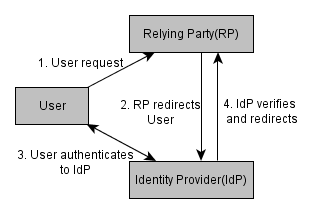
\includegraphics[width=0.5\textwidth]{Picture.png}
  \caption{Temporary figure}
  \label{fig:SSOFlow}
\end{figure}

\section{Result} % 200
    The weights
    Graphed results and average?

\section{Analysis/Conclusion} % 200
    Does it perform "not-so-good" at some sequences?


    Citation example: ~\cite{BillionKeys}.


\begingroup
  \raggedright
  \bibliography{bibliography}
  \bibliographystyle{ieeetr}
\endgroup

\end{document}


